\documentclass{beamer}
\mode<presentation>
{
  \usetheme{default}      % or try Darmstadt, Madrid, Warsaw, ...
  \usecolortheme{default} % or try albatross, beaver, crane, ...
  \usefonttheme{default}  % or try serif, structurebold, ...
  \setbeamertemplate{navigation symbols}{}
  \setbeamertemplate{caption}[numbered]
} 
\usepackage[english]{babel}
\usepackage[utf8x]{inputenc}
\usepackage[T1]{fontenc}
\usepackage{amsmath}
\usetheme{Antibes}
\usepackage{centernot}
\usepackage{hyperref}
\usepackage{tabularx}
\usepackage{dsfont}
\usepackage{natbib}
\usepackage{breqn}
\usepackage[acronym,nonumberlist,nopostdot,toc]{glossaries}
\usepackage{upgreek}
\usepackage{arydshln}
\usepackage{algorithm}
\usepackage{algorithmicx}
\usepackage{algpseudocode}
\usepackage{float}
\usepackage{amssymb}
\usepackage{geometry}
\usepackage{amsmath}
\usepackage{graphicx}
\usepackage{tabto}
\usepackage[justification=centering]{caption}
\expandafter\def\expandafter\insertshorttitle\expandafter{%
   \insertshorttitle\hfill%
   \insertframenumber\,/\,\inserttotalframenumber}   
\newcommand{\R}{\mathbb R} % Beispiel für die Definition eines eigenen Befehls

\graphicspath{{figures/01/}}

\title[]{Introductory Course: Machine Learning (WWI15B4)}
\vspace{3cm}
\subtitle{Introduction}
\author{Fabio Ferreira, David Bethge}
\institute{DHBW Karlsruhe}
\date{}

\begin{document}

\begin{frame}
  \titlepage

\end{frame}
\begin{frame}{Outline}
  \tableofcontents
\end{frame}




\section{About us and Administrative}


\begin{frame}{About us}

\begin{columns}
\begin{column}{0.35\textwidth}
   \begin{figure}
	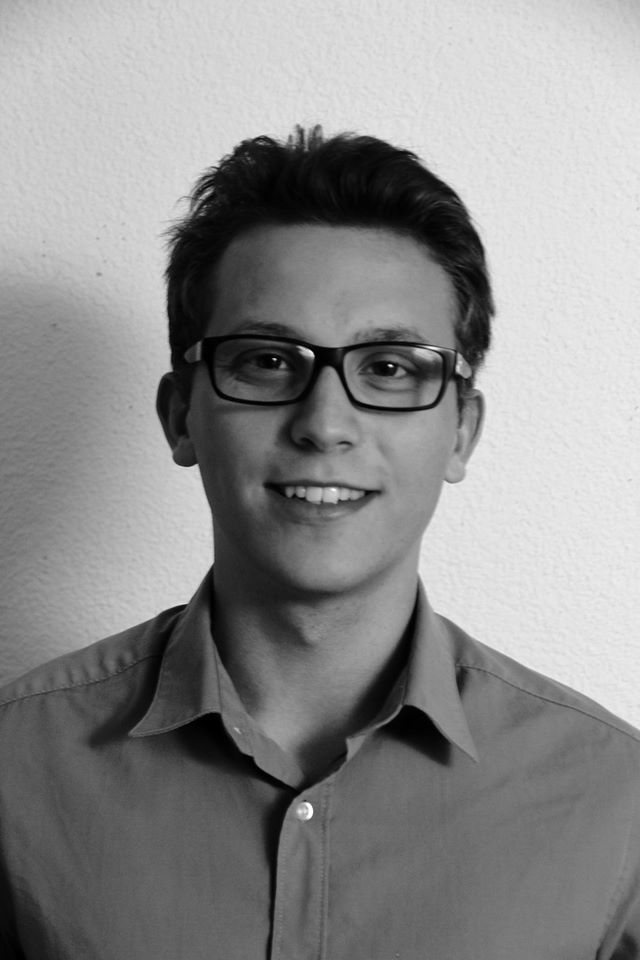
\includegraphics[width=0.6\linewidth]{david_black_and_white}
	\caption*{David Bethge}
\end{figure}
\end{column}
\begin{column}{0.65\textwidth}  %%<--- here
    \begin{itemize}
	\item \textbf{background}: Industrial Engineering with focus on data science
	\item \textbf{interests}: Machine Learning, intelligent driving
	\item \textbf{experience}: various ML applications e.g.:
    \begin{itemize}
    \item analytics of car logging data 
    \item life-cycle risk measures for power plants 
    \item ML for automatic building of virtual cars
    \item predictive maintenance for robots 
    \end{itemize}
	\item \textbf{research interests}: robust statistical learning, perception, learning embeddings

\end{itemize}
\end{column}
\end{columns}
\end{frame}




\begin{frame}{About us}

\begin{columns}
\begin{column}{0.35\textwidth}
   \begin{figure}
	
\includegraphics[width=0.6\linewidth]{fabio_bw}
	\caption*{Fábio Ferreira}
\end{figure}
\end{column}
\begin{column}{0.65\textwidth}  %%<--- here
    \begin{itemize}
	\item \textbf{background}: CS with focus on Machine Learning (ML)
	\item \textbf{interests}: ML/ML for robotics, computer vision, reinforcement learning (RL)
	\item \textbf{experience}: various ML applications e.g.:
    \begin{itemize}
    \item deep auto encoders for video processing
    \item DNN architecture evaluation 
    \item DNN vs. kernel methods in finance
    \end{itemize}
	\item \textbf{research interests}: fundamental ML without specific applications, 	cognitive robotics (e.g. advance artificial reasoning/world understanding through DNN)
    
\end{itemize}
\end{column}
\end{columns}
\end{frame}

\begin{frame}{Lecture Overview}
[see Syllabus]
\end{frame}

\begin{frame}{Course Material}
\begin{itemize}
\item course material on Moodle\\
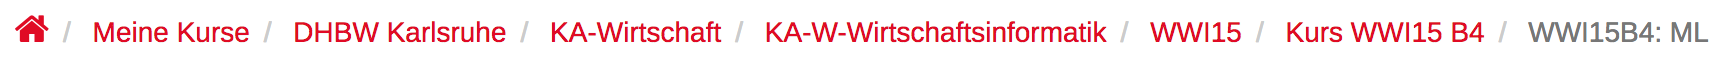
\includegraphics[width=1\textwidth]{moodle_path}
\item obtain feedback about enrollment
\end{itemize}

\end{frame}

\begin{frame}{Lecture Overview}
\begin{itemize}
\item May 8: \tabto{2cm} Introduction
\item May 16: \tabto{2cm} Statistical Learning (1)
\item May 24: \tabto{2cm} Concept Learning
\item May 29: \tabto{2cm} Statistical Learning (2)
\item June 6: \tabto{2cm} Classification (1)
\item June 12: \tabto{2cm} Classification (2) (3)
\item June 20: \tabto{2cm} Clustering
\item July 3: \tabto{2cm} Outlook
\end{itemize}
No lecture in week June 25-29
\end{frame}

\begin{frame}{Lecture Overview}
\begin{itemize}
\item May 8: \tabto{2cm} Introduction
\item \textbf{May 16: \tabto{2cm} Statistical Learning (1) (3h15)} (1pm-4:15)
\item May 24: \tabto{2cm} Concept Learning
\item May 29: \tabto{2cm} Statistical Learning (2)
\item June 6: \tabto{2cm} Classification (1)
\item \textbf{June 12: \tabto{2cm} Classification 2(+3) (2h30)} (10:45am-1:15pm)
\item June 20: \tabto{2cm} Clustering
\item July 3: \tabto{2cm} Outlook
\end{itemize}
\end{frame}

\begin{frame}{Exam / Exam Allocation}
\begin{center}
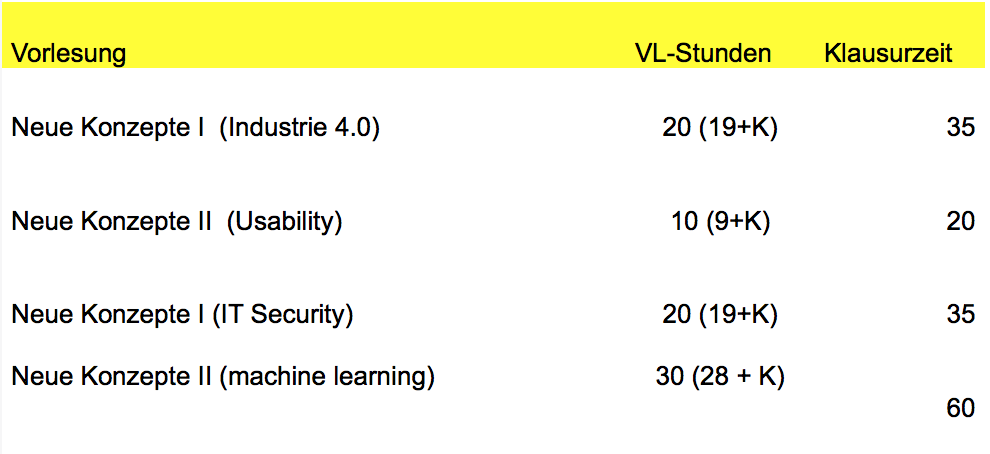
\includegraphics[width=0.8\textwidth]{klausurplan}
\end{center}
Exam date: July 23, 10am - 12:30pm
\end{frame}



\begin{frame}{Recommended Literature}
\begin{center}

\includegraphics[width=0.5\textwidth]{qr_code_reading}
\end{center}
or: \url{https://goo.gl/3ogHU4}
% pw on the board
\end{frame}

\begin{frame}
\frametitle{contact}
\textbf{email:}
\begin{itemize}
\item Fabio Ferreira: ferreira.fabio@edu.dhbw-karlsruhe.de
\item David Bethge: bethge.david@edu.dhbw-karlsruhe.de
\end{itemize}

\end{frame}





\section{Introduction}
\subsection{Motivation and Introduction}
	\begin{frame}{Applications}
		\begin{itemize}
			\item Automotive
			\item Bioinformatics
			\item Computer Vision
			\item Games
			\item Financial markets
			\item Linguistics and Speech
			\item Insurance
			\item Marketing
			\item Object recognition
			\item Optimization
			\item Robotics
			\item Search engines
			\item ...
		\end{itemize}
	\end{frame}

	\begin{frame}{What is learning actually?}
		\begin{itemize}
			\item \textit{"Learning denotes changes in the system that are adaptive in the sense that they enable the system to do the same task or tasks drawn from the \textbf{same population more efficiently and more effectively} the next time."} - Herbert A. Simon
			\item Knowledge: "Interpretation of the information contained in data" (Kononekno, Matjazkukar, 2007)
		\end{itemize}
	\end{frame}
	
	\begin{frame}{Machine Learning - Definition}
		\begin{itemize}
			\item Tom M. Mitchell: "A computer program is said to learn from experience E with respect to some class of tasks T and performance measure P if its performance at tasks in T, as measured by P, improves with experience E."
			\item T: Playing checkers game, E: Played games, P: Percentage of won games
		\end{itemize}
        \begin{figure}
        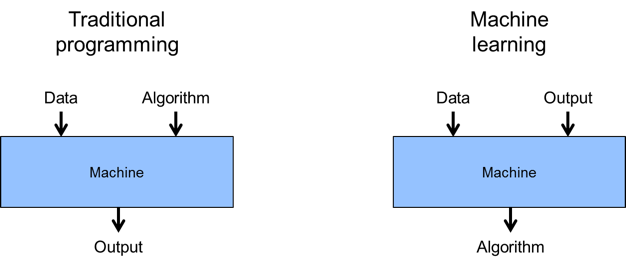
\includegraphics[width = 0.7\linewidth]{figures/introduction/MachineLearningTalend2}
        \end{figure}
        
        
	\end{frame}

	\begin{frame}{Machine Learning - Overview}
		\begin{itemize}
			\item Learning from data and making predictions or decisions on data
			\item Not explicitly, static programmed
			\item Computer programs, that automatically improve with experience
			\item Goal: Ability to perform accurately on new, unseen data, after learnt from a training data set.
			\item Knowledge base is needed
			\item Problem: How well does the training experience represents the distribution of examples?
			\item Problem: Why did the computer decided this way?
		\end{itemize}
	\end{frame}
	
	\begin{frame}{Machine Learning - Overview}
		\begin{itemize}
			\item Often uses statistical and mathematical optimization techniques
			\item Learning problems often formulated as minimization problems, using a loss function, expressing a discrepancy between prediction and training data.	
			\item Direct vs. indirect training feedback
		\end{itemize}
	\end{frame}
	
	\begin{frame}{Machine Learning - Data Mining}
		\begin{itemize}
			\item Data Mining: Overlap with Machine Learning but only focusing on data analysis
			\item Machine Learning: Prediction, based on known properties
			\item Data Mining: Discovery of unknown properties
			\item Uncover hidden insights
			\item Dimensional reduction
		\end{itemize}
	\end{frame}
	
	\begin{frame}{Why now?}
		\begin{itemize}
			\item Most ideas from the second half of the 20th century
			\item Today: \textbf{Availability of data and possibility to do large computation cheaply}
		\end{itemize}
	\end{frame}
	
	\begin{frame}{A little bit of history}
		\textit{It is virtually impossible to find an 'original' idea that was not present earlier in the scientific literature. When the need for an idea is in the air, the idea is usually discovered by several groups simultaneously"} - James A. Anderson
	\end{frame}	
	
	\begin{frame}{A little bit of history}
		\begin{itemize}
			\item 1941: Zuse Z3
			\item Arthur Samual, 1959 (at IBM): Program, that played checkers better than himself (based on rules and probabilities)
			\item Modeling of Neurones (Rosenblatt 1958)
		\end{itemize}
	\end{frame}	
	
	\begin{frame}{A little bit of history}
		\begin{itemize}
			\item 1955-1968: Begin
			\item 1969-1979: "Depression" (XOR-Problem)
			\item 1979-1986: "Renaissance" (Various methods)
			\item since 1986: Extensions, more complex systems...
			\item today: Attempts to explain why a system does what it does.
		\end{itemize}
        \begin{figure}
        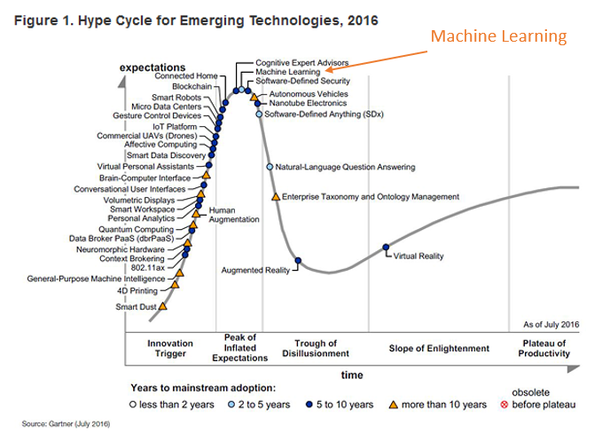
\includegraphics[width = 0.7\linewidth]{figures/introduction/HypeCycle}
        \end{figure}
	\end{frame}	


    

	
\subsection{Classification criteria: Machine Learning}
	\begin{frame}{Classification criteria: Machine Learning}
		 \begin{tabular}{lcc}
		 	\hline
			\textbf{Type of Inference}	& inductive 	& deductive\\
			\textbf{Learning approach}	& symbolic	 	& non-symbolic\\
			\textbf{Types of learning}	& supervised	& unsupervised\\
			\textbf{Example usage}		& incremental	& non-incremental\\
			\textbf{Extent of examples}	& extensive		& little\\
			\textbf{Background knowledge}& empirical	 	& axiomatic\\
			\hline
		 \end{tabular}
	\end{frame}
	
	\begin{frame}{Type of Inference}
		\begin{itemize}
			\item Inductive: Specific to general: Making generalizations from specific, available observations.
			\item Deductive: General to specific: Based on a theory or formulas we can make a prediction: "Syllogism"
			\newline
			\item Example inductive: {"Jim is a man", "Jim is mortal"} $\rightarrow$ "All men are mortal"
			\item Example deductive: {"All men are mortal", "Jim is a man"} $\rightarrow$ "Jim is mortal"
		\end{itemize}
	\end{frame}

	\begin{frame}{Learning approach}
    \begin{small}
		\begin{itemize}
			\item Symbolic: Using human-readable information related to what you think is necessary. The reasoning process can be easily understood. Rules and knowledge has to be hand coded
			\item Non-symbolic: Feeding in raw information that can be analyzed and then implicit knowledge can be constructed. It is often difficult to understand how the system came to a conclusion
			\newline
			\item Example symbolic: ontology, taxonomy, rule-based knowledge representations
			\item Example non-symbolic: matrices, scalars or vectors
		\end{itemize}
        \end{small}
	\end{frame}

	\begin{frame}{Types of learning}
		\begin{itemize}
			\item \textbf{Supervised}: With labeled data, with input and output variables
			\item \textbf{Unsupervised}: Without labeled data, without an output variable
			\newline
			\item Example supervised: Classification: Decide whether a picture shows a man or a woman 
			\item Example unsupervised:	Model underlying structure: Clustering: Grouping customers by purchasing behavior
		\end{itemize}
	\end{frame}
    \begin{frame}
    \begin{figure}
        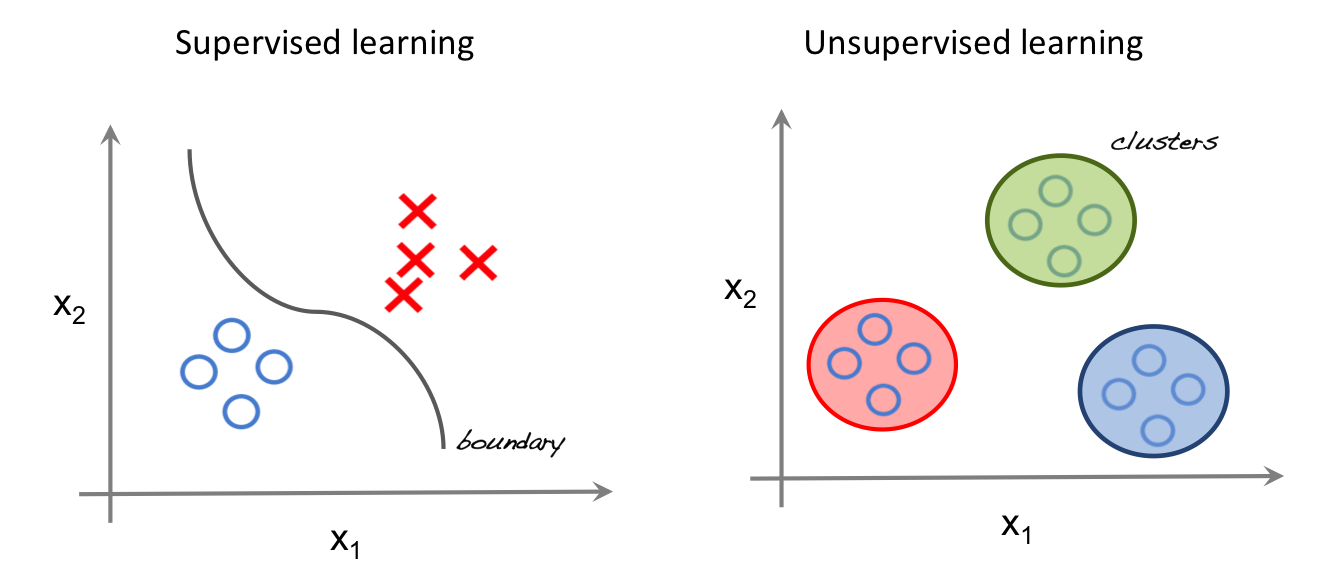
\includegraphics[width = .9\linewidth]{figures/introduction/supervised_unsupervised}
    \end{figure}
    \end{frame}
    
    \begin{frame}
        \begin{figure}
            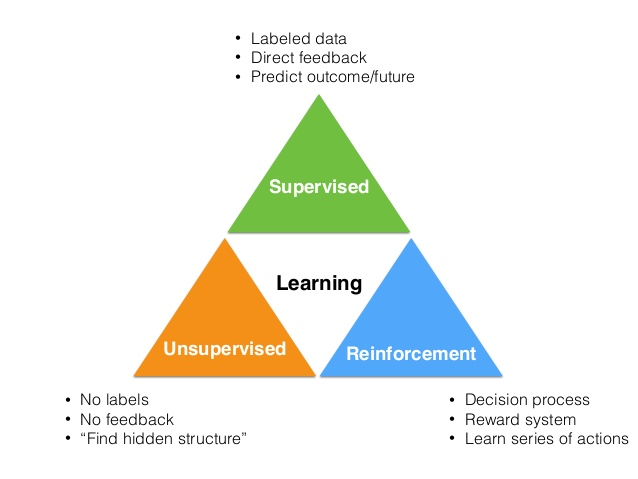
\includegraphics[width = .9\linewidth]{figures/introduction/type_machine_learning}
    \end{figure}
    \end{frame}

	\begin{frame}{Example usage}
    	\begin{small}
		\begin{itemize}
			\item Incremental: Training data can be severally/successively inserted and the system improves with each example the hypotheses.
			\item Non-incremental: All data have to be inserted at once.
			\newline
			\item Example incremental: Adding new rules based on new examples, which do not affect the old rules based on the old examples: \newline \{"All men are mortal", "Jim is a man"\} $\rightarrow$ "Jim is mortal" \newline \{"All dogs are mortal", "Garfield is a dog"\} $\rightarrow$ "Garfield is mortal"
			\item Example non-incremental: Clustering a group of people by their salary. If one person with a really different salary is added, all other persons have to be clustered again.
		\end{itemize}
        \end{small}
	\end{frame}

	\begin{frame}{Background knowledge}
		\begin{itemize}
			\item Empirical: Statistical analyzed know-how
			\item Axiomatic: Logic deductions
		\end{itemize}
	\end{frame}
	
	\begin{frame}{Classification criteria: Machine Learning}
		 \begin{tabular}{lcc}
		 	\hline
			\textbf{Type of Inference}	& inductive 	& deductive\\
			\textbf{Learning approach}	& symbolic	 	& non-symbolic\\
			\textbf{Types of learning}	& supervised	& unsupervised\\
			\textbf{Example usage}		& incremental	& non-incremental\\
			\textbf{Extent of examples}	& extensive		& little\\
			\textbf{Background knowledge}& empirical	 	& axiomatic\\
			\hline
		 \end{tabular}
	\end{frame}  
	
	
\begin{frame}
\frametitle{Skillset}
\begin{figure}
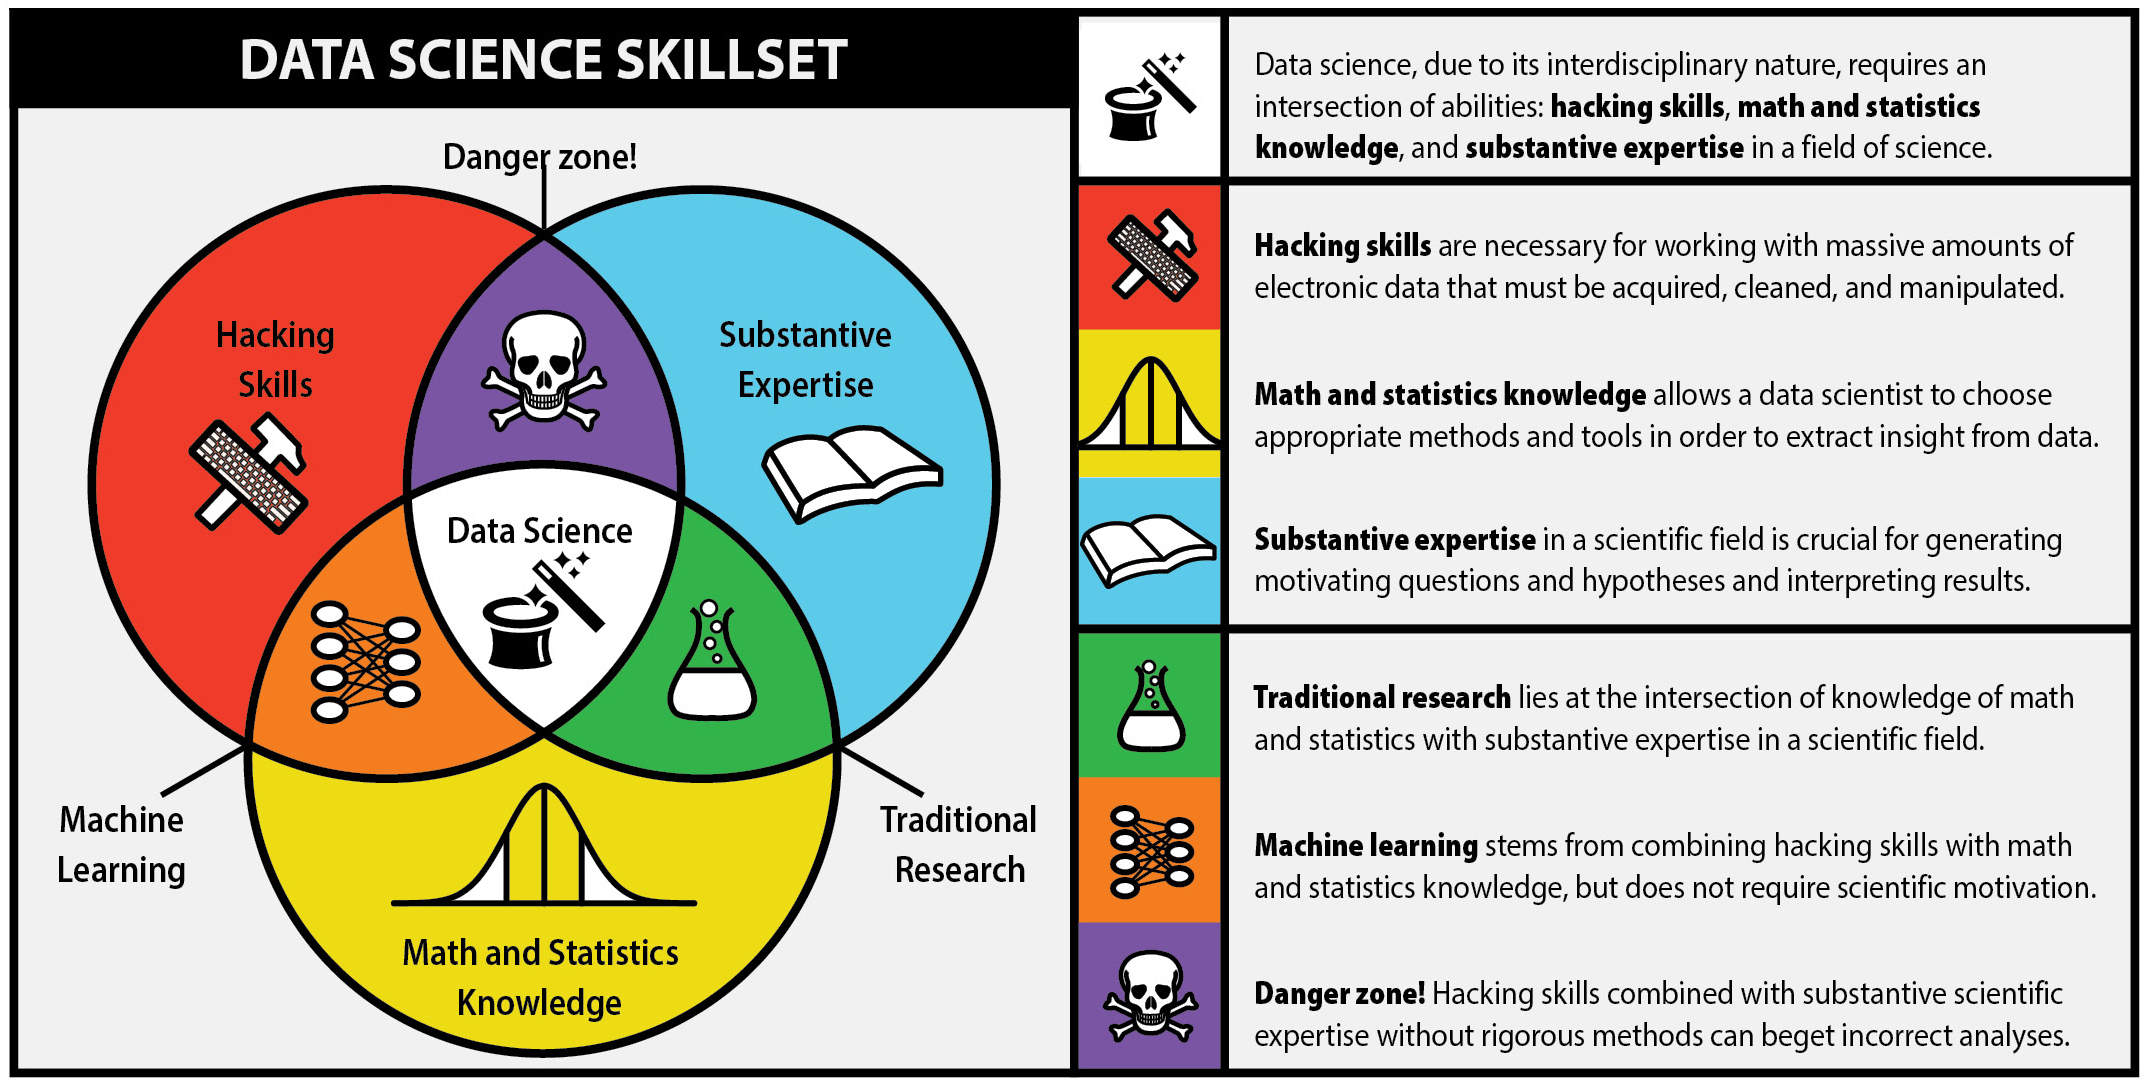
\includegraphics[width = 1\linewidth]{figures/introduction/data_science_skillset}
\end{figure}
\end{frame}
	
	
	
\subsection{Types of Data}
\begin{frame}{Types of data}
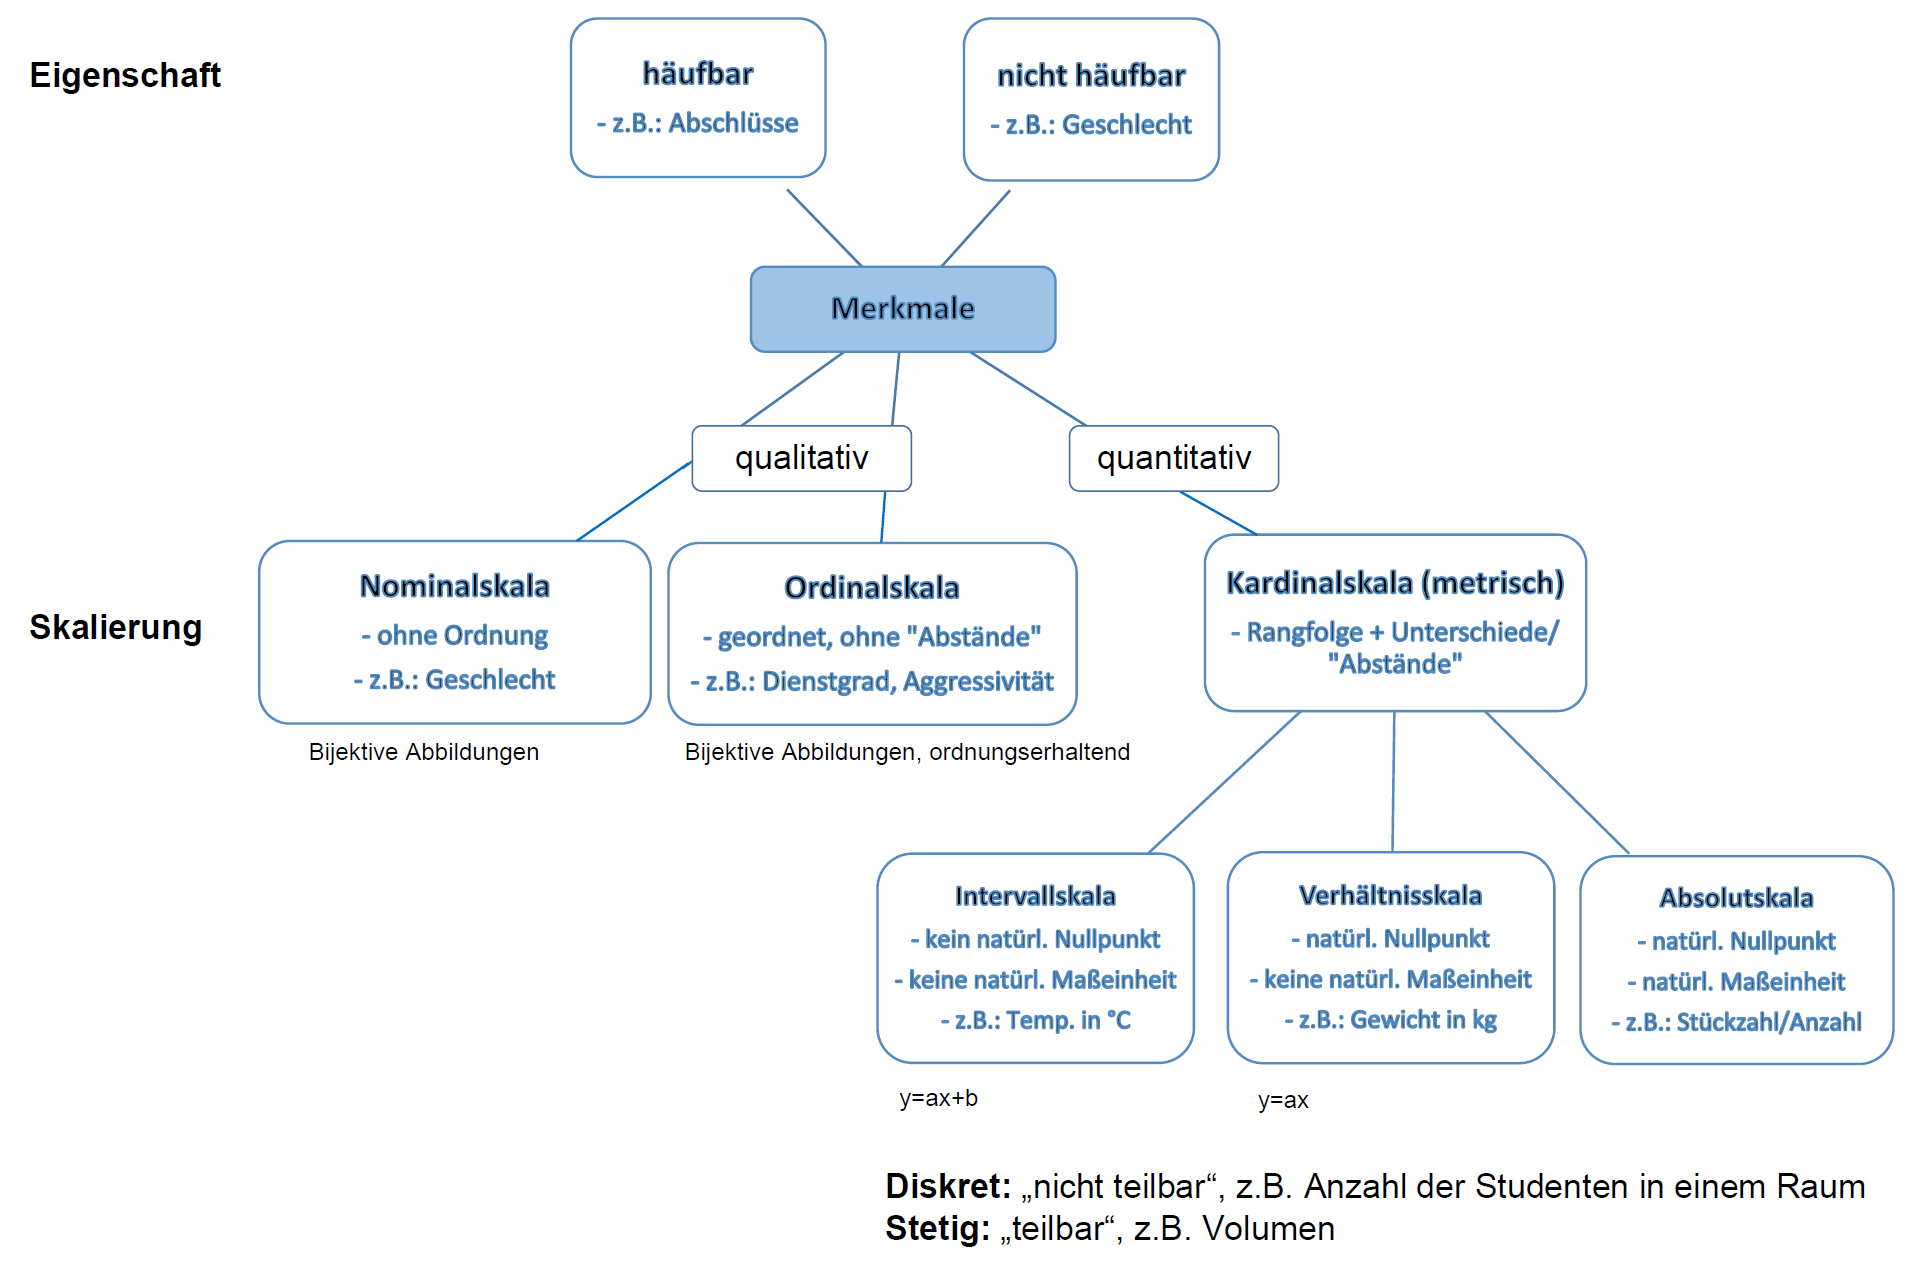
\includegraphics[width=1\textwidth]{figures/introduction/variables}
\end{frame}	    

\subsection{CRISP-DM}
	\begin{frame}{Machine Learning Approach: CRISP-DM}
    \textbf{How is a machine learning project done in practice?} 
		\begin{itemize}
			\item Cross Industry Standard Process for Data Mining
			\item 1997: Founded by the European Commission
			\item 1996: DaimlerChrysler, SPSS, NCR
			\item Today: IBM
		\end{itemize}
	\end{frame}

	\begin{frame}{CRISP-DM}
    \begin{center}
    		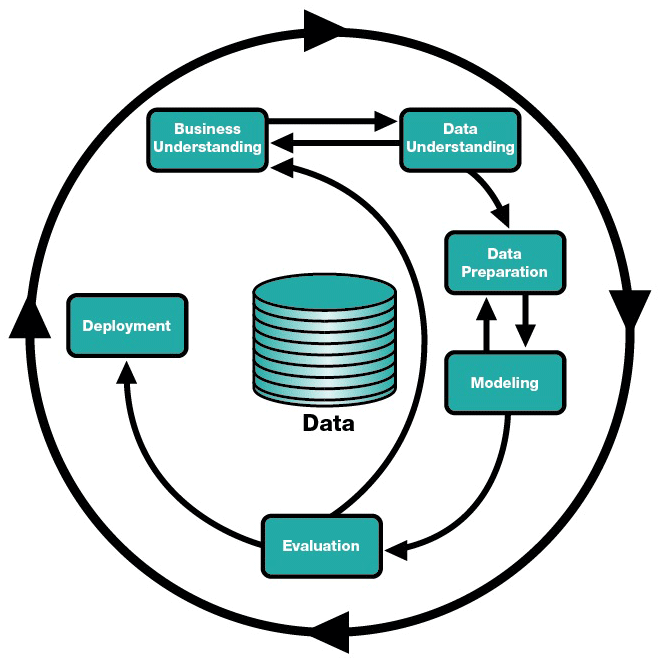
\includegraphics[width=0.6\textwidth]{figures/introduction/newcrispdiagram.png}
    \end{center}
	\end{frame}
	
	\begin{frame}{Business Understanding}
		What does the customer want to accomplish?
		\begin{itemize}
			\item Uncover important facts
			\item Record information about the business situation
			\item Describe primary and related business goals
		\end{itemize}
        \bigskip
		Produce Project Plan
		\begin{itemize}
			\item Describe the plan to achieve the data mining goals
			\item Describe success criteria
		\end{itemize}
	\end{frame}
    
	\begin{frame}{Business Understanding}
		Go into detail
		\begin{itemize}
			\item List available resources
			\item List requirements, assumptions and constraints
			\item List risks and alternatives
		\end{itemize}
        \bigskip
		Costs and benefits
		\begin{itemize}
			\item Do a cost-benefit analysis
		\end{itemize}
        \bigskip
		Determine Data Mining Goals
	\end{frame}
	
	\begin{frame}{Data Understanding}
		\begin{itemize}
			\item Where is the needed data?
			\item What: restrictions, type, structure, date, \dots
			\item Quality: accuracy (outliers), completeness (missing values), consistency (errors)
		\end{itemize}
	\end{frame}
	
		\begin{frame}{Data Understanding}
			\begin{itemize}
				\item Collect data
				\item Write data collection report
				\item Describe data
				\item \textbf{Explore Data: Analyze, visualize (scatter-plot, histogram etc.} 
				\item Examine the quality of the data
				\item Data exploration and quality report
			\end{itemize}
            \begin{figure}
            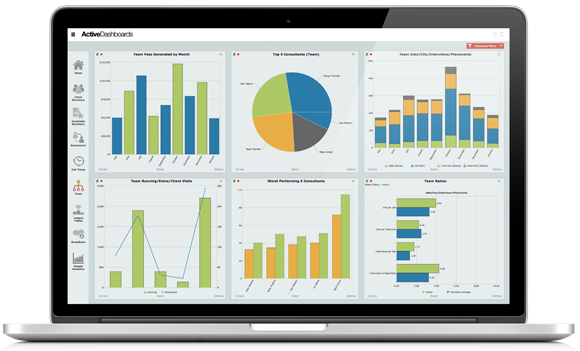
\includegraphics[width = 0.5\linewidth]{figures/introduction/data_understanding}
            \end{figure}
		\end{frame}
	
	\begin{frame}{Data Preparation}
		\begin{itemize}
			\item \textbf{Goal}: Dataset that can be used to model (apply machine learning algorithms)
		\end{itemize}
        \begin{figure}
        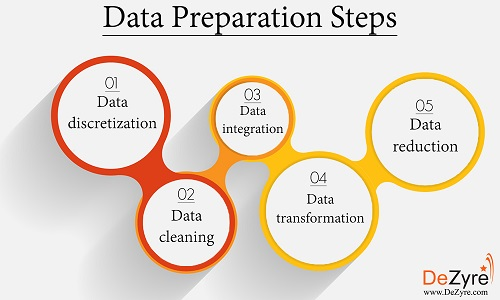
\includegraphics[width = .7\linewidth]{figures/introduction/data_prep}
        \end{figure}
	\end{frame}
	
		\begin{frame}{Data Preparation: Selection}
			\begin{itemize}
				\item Merge data if necessary
				\item Select attributes as well as observations
				\item Observations: Sampling with or without replacement
				\item Observations: Systematic sampling, stratified sampling, bootstrap sampling
				\item Attributes: Select subset, missing values,too much or too little variation, correlations, \dots
				\item Attributes: Dimension reduction
               \end{itemize}
		\end{frame}

		\begin{frame}{Data Preparation: Selection}
			Filter vs. Wrapper vs. Embedded techniques
            \begin{itemize}
				\item Filter: Evaluation of attributes independent of modeling technique
				\item Wrapper: Using performance of learning method for evaluation
				\item Embedded techniques: Attribute selection part of the method
			\end{itemize}
		\end{frame}

		\begin{frame}{Data Preparation: Cleaning}
			\begin{itemize}
				\item Check for missing values, inaccurate data, duplicates, outliers, \dots
				\item Deal with errors by selecting a clean subset or replacing errors			
			\end{itemize}
            \bigskip
			Missing Values
			\begin{itemize}
				\item Ignore
				\item Replace with the most common attribute value
				\item Replace with the most common attribute value of the same class
				\item Try to model: Use for example probability distribution
            \end{itemize}
		\end{frame}
		
		\begin{frame}{Data Preparation: Construction and Transformation}
			\begin{itemize}
				\item Transform data (e.g. year of birth to age)
				\item Construct derived attributes (e.g. PCA) or observations (sampling e.g. bootstrap)
			\end{itemize}
		\end{frame}	
	
	\begin{frame}{Modeling}
		\begin{itemize}
			\item Select concrete modeling technique
			\item Record model assumptions
			\item Describe how to and separate data into training, validation and test data 
			\item \textbf{Run model}
			\item List parameter settings
			\item Describe produced model with interpretation and difficulties
			\item Run different models and compare them: Different parameters and/or different methods 
			\item Summarize results
		\end{itemize}
	\end{frame}

	\begin{frame}{Evaluation}
		\begin{itemize}
			\item Evaluate models with respect to the business objectives
			\item Review the whole process: Are the models correctly built? Were only attributes used that will also be available in the future?
			\item Decide how to proceed and document everything
		\end{itemize}
	\end{frame}

	\begin{frame}{Deployment}
		\begin{itemize}
			\item Describe deployment plan
			\item Plan and summarize monitoring and maintenance
			\item Final report
			\item Review project, document and learn for future projects
		\end{itemize}
	\end{frame}	

	\begin{frame}{CRISP-DM}
    \begin{center}
    		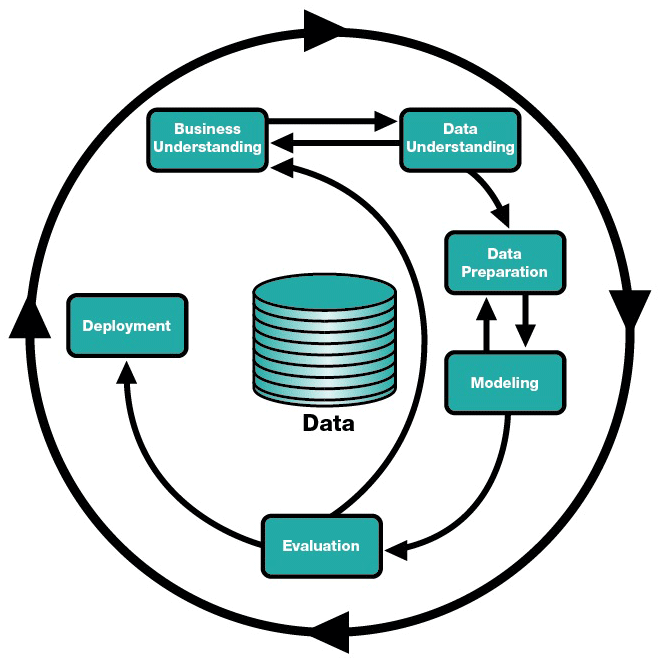
\includegraphics[width=0.6\textwidth]{figures/introduction/newcrispdiagram.png}
    \end{center}
	\end{frame}
    

	
	
\subsection{Notation}
	\begin{frame}{Notation}
		Data matrix X \\
        For supervised learning: Output matrix Y \\
        n: number of observations: $i\in\{1,\dots,n\}$ \\ 
        p: number of attributes: $j\in\{1,\dots,p\}$ \\
        \bigskip
        $Y=\begin{pmatrix}
        y_{1} \\
		\vdots \\
        y_{i} \\
        \vdots \\
        y_{n}\\
        \end{pmatrix}$ \qquad  
        $X=\begin{pmatrix}
        x_{11} & \dots & x_{1j} & \dots & x_{1p} \\
		\vdots & {}	   & \vdots & {}    & \vdots \\
        x_{i1} & \dots & x_{ij} & \dots & x_{ip} \\
        \vdots & {}	   & \vdots & {}    & \vdots \\
        x_{n1} & \dots & x_{nj} & \dots & x_{np} \\
        \end{pmatrix}=
        \begin{pmatrix}
        X_{(1)} \\
		\vdots \\
        X_{(i)} \\
        \vdots \\
        X_{(n)}\\
        \end{pmatrix}$  \\
        \bigskip
        For simplicity: $X_{(i)}=x_i$
	\end{frame}

	


\subsection{Learning Theory}
	\begin{frame}{Learning Theory}
		\begin{itemize}
			\item Shortcut of Fabios and Davids 4th chapter.
		\end{itemize}
	\end{frame}

	


\subsection{Overview methods}
	\begin{frame}{Overview methods}
    \begin{tiny}
		\begin{tabular}{l|cc|cc|cc|}
			\hline
		    {}			& \multicolumn{2}{c}{Inference} & \multicolumn{2}{c}{Learning approach} & \multicolumn{2}{c}{Types of learning}  \\
			Methods		& inductive & deductive			& symb. & non-symb.		& sup. & unsup. \\ \hline
            Regression  & x & {}   & x & {}   & x & {}    \\ \hline
            Decision Tree & x & {}  & x & {}  & x & {}  \\ \hline
            K-nearest neighbors & x & {}  & {} & x  & x & {}  \\ \hline
            SVM  & x & {}  & {} & x  & x & {}  \\ \hline
            K-means (clustering)  & x & {}  & {} & x  & {} & x  \\ \hline
            PCA & x & {}   & x & {}   & {} & x   \\ \hline
            NN  & x & {}  & {} & x  & x & {}  \\
			\hline
		\end{tabular} \\ 
        \bigskip
        \bigskip
        \begin{tabular}{l|cc|cc|cc|}
			\hline
		    {}		 & \multicolumn{2}{c}{Example usage} & \multicolumn{2}{c}{Extent of examples} & \multicolumn{2}{c}{Background knowledge} \\
			{}	& incr. & non-incr. 	& extensive & little		& empirical & axiomatic\\ \hline
            Regression   & {} & x  & x & {}  & x & {} \\ \hline
            Decision Tree & x & x  & x &  {} & x & {} \\ \hline
            K-nearest neighbors & {} & x  & x & {}  & x & {}\\ \hline
            SVM  & {} & x  & x & {}  & x & {}\\ \hline
            K-means (clustering)  & {} & x  & x & {}  & x & {}\\ \hline
            PCA & {} & x  & x & {}  & x & {} \\ \hline
            NN & {} & x  & x & {}  & x & {}\\
			\hline
		\end{tabular}
    \end{tiny}
	\end{frame}
    
    
    \begin{frame}
    \frametitle{Reading assignment}
    Next lecture we will need some basic matrix algebra.
    
    
    \end{frame}
    
\end{document}